
La siguiente planificación económica tiene en cuenta los siguientes puntos:
\begin{itemize}
\item[•]El proyecto no esta orientado a dar rentabilidad económica.
\item[•]Todas las tareas se asignaran a la misma persona, el sueldo se supondrá según el rol que asuma en cada momento. 
\end{itemize}

\subsection{Identificación y estimación de costes}
\subsubsection{Costes de personal}
A pesar que el proyecto solo sera desarrollado por una única persona, durante el transcurso del proyecto asumirá diferente roles. Los costes de personal se estimaran calculando la carga de trabajo que tendrá que asumir cada rol, se establecerá el coste por hora a cada rol.

Basándonos a la planificación temporal:
\begin{itemize}
\item La parte que corresponde a planificación, que va del día 09/14/2015 al 11/14/15, sera asignada al jefe del proyecto.
\item Durante los \textit{sprints}, del 11/15/15 al 04/09/16, la carga de trabajo se distribuirá entre todos los roles, de la siguiente manera:
\begin{description}
\item[Jefe del proyecto o Scrum master] 15\%
\item[Programador] 70\%
\item[Tester] 15\%
\end{description}
\item La ultima fase donde se preparara la presentación del proyecto estará asignada al jefe del proyecto, del 04/10/16 al 04/20/16.
\end{itemize}

La carga de trabajo de las fases esta especificada en la planificación \ref{sec:planificacion}. A continuación en la tabla \ref{tab:cost_tab} se muestra la estimación de costes de personal. Para hacer el calculo de las horas de trabajo se ha tenido en cuenta la estimación temporal de la planificación y la distribución del trabajo realizada previamente.

\begin{table}
\setlength{\arrayrulewidth}{1mm}
\setlength{\tabcolsep}{12pt}
\renewcommand{\arraystretch}{2.5}
{
\begin{tabular}{ |p{2cm}|p{2cm}|p{2cm}|p{2cm}|}
\hline
\multicolumn{4}{|c|}{Costes de personal} \\
\hline
ROL &Horas & \euro /hora &Coste total \\
\hline
Jefe del proyecto &212.6 &40 & 8504\\
Programador &163.8 &30 & 4914\\
Sistemas &33.6 &25 &840\\
&&& 14258\\
\hline
\end{tabular}
}
\caption{Tabla de costes de personal}
\label{tab:cost_tab}
\end{table}
\newpage
\subsubsection{Coste del espacio de trabajo}

Bajo el supuesto que se desarrollase el proyecto en un área de \textit{coworking}, concretamente en MG CoWorking (BRUC), situado en la calle del Bruc, el coste seria de 100\euros al mes, dado que el proyecto dura aproximadamente 7 meses, tal como podemos ver en la planificación temporal\ref{sec:planificacion}, implicaría un coste de 700\euros.

\subsubsection{Coste del los servidores}
Suponiendo que durante la fase de \textit{deploy} se alquilaran servidores de Digital Ocean, el precio es de 10\euros al mes, dado que la fase de deploy dura un mes el coste sera de 10\euros .\\
\begin{figure}[ht!]
	\center
	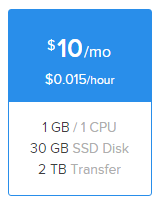
\includegraphics[scale=1.0]{add/do_server.PNG}
	\label{fig:Precio y especificaciones del servidor}
	\caption{Coste del alquiler de un servidor en DigitalOcean}
\end{figure}
\newpage

\subsubsection{Valoración}
Dado que es un proyecto de carácter académico sin pretensiones comerciales y que se ha decidido por cuestiones tanto técnicas como éticas usar open source para su desarrollo, este apartado puede quedar levemente desdibujado, dadas estas circunstancias. Si bien es cierto que uno de los grandes potenciales de las TIC es el poder crear un valor añadido muy alto partiendo de unos costes de producción muy bajos.

\section{Sostenibilidad y compromiso social}
Cada una de las tres secciones siguientes están evaluadas sobre 10.
\subsection{Dimensión económica - 7}
El proyecto a desarrollar no busca la rentabilidad económica, por otro lado sus costes de desarrollo son muy bajos, siendo un proyecto muy viable económicamente. Si bien, en el caso de querer comercializar el software, como hemos podido ver en el estado del arte, es difícil que en el tiempo de duración del proyecto con los recursos que se disponen dar una solución del nivel de las soluciones actuales.
\subsection{Dimensión social - 9}
Al ser un software en el que todo su código sera abierto y integrara varias tecnologías que actualmente siguen en desarrollo, podrá ayudar a varias comunidades de desarrolladores. Por otro lado un resultado final del proyecto podría ser interesante para diferentes sectores dedicados a la genealogía que busquen una solución abierta para guardar la información de la que disponen.
\subsection{Dimensión ambiental - 6}
El proyecto tiene un mínimo impacto medio ambiental, no se espera que mediante el uso del software se ahorre ningún recurso material, pero el coste de mantenimiento y creación no implica consumir recursos materiales.